%\documentclass{llncs}
%\NeedsTeXFormat{LaTeX2e}[1995/12/01]
\documentclass[10pt]{bmc_article}
\usepackage{cite} % Make references as [1-4], not [1,2,3,4]
\usepackage{url}  % Formatting web addresses  
\usepackage{ifthen}  % Conditional 
\usepackage{multicol}   %Columns
\usepackage[utf8]{inputenc} %unicode support
\usepackage{listings}

%\usepackage[applemac]{inputenc} %applemac support if unicode package fails
%\usepackage[latin1]{inputenc} %UNIX support if unicode package fails
\urlstyle{rm}

%Shaded framed
\usepackage{framed,color}
\definecolor{shadecolor}{rgb}{0.96,0.96,0.96}

%\def\includegraphic{}
%\def\includegraphics{}
\usepackage{graphicx}

\setlength{\topmargin}{0.0cm}
\setlength{\textheight}{21.5cm}
\setlength{\oddsidemargin}{0cm} 
\setlength{\textwidth}{16.5cm}
\setlength{\columnsep}{0.6cm}

\newboolean{publ}
\newenvironment{bmcformat}{\begin{raggedright}\baselineskip20pt\sloppy\setboolean{publ}{false}}{\end{raggedright}\baselineskip20pt\sloppy}

\lstdefinelanguage[1.1]{sparql}{morekeywords={PREFIX,SELECT,CONSTRUCT,WHERE,ASK,DESCRIBE,A,NOT,EXISTS,FILTER,regex},sensitive=true,morestring=[s]{<>},morestring=[s]{""},escapeinside={~}{~},extendedchars=true,morecomment=[l]{\#}}
\lstset{
  basicstyle=\small, % print whole listing small
  identifierstyle=, % nothing happens
  commentstyle=\color{blue}, % white comments
  stringstyle=\ttfamily, % typewriter type for strings
  showstringspaces=false
  numbers=left, 
  numberstyle=\tiny,
  numberbychapter=true,
  xleftmargin=0.1\linewidth,
  xrightmargin=0.1\linewidth,
  boxpos=c,
  frame=, 
  numbersep=2p,
  columns=fullflexible,
  escapechar=`
}

%\newfloat{example}{h}{ttl}[section]
%\floatname{example}{Example}		
\begin{document}
\begin{bmcformat}
\title{Semantic standard for describing the location of nucleotide and protein feature annotation.}
\author{Jerven Bolleman\correspondingauthor$^{1}$\email{Jerven Bolleman\correspondingauthor - jerven.bolleman@isb-sib.ch}%
    \and Christopher J Mungall$^{2}$%
    \and Francesco Strozzi$^{3}$%
    \and Joachim Baran$^{4}$%
    \and Michel Dumontier$^{5}$%
    \and Raoul J. P. Bonnal$^{6}$%    
    \and Robert Buels$^{7}$%
    \and Robert Hoehndorf$^{8}$%
    \and Takatomo Fujisawa$^{9}$%
    \and Toshiaki Katayama$^{10}$%
    \and Peter J. A. Cock$^{11}$%
%
}
\address{
 \iid(1) SIB Swiss Institute of Bioinformatics, Centre Medical Universitaire, 1 rue Michel
Servet, 1211 Geneva 4, Switzerland,
 \iid(2) Genomics Division, Lawrence Berkeley National Laboratory, Berkeley, CA, 94720, US
 \iid(3) CeRSA, Parco Tecnologico Padano, Lodi 26900, Italy, and
 \iid(4) Ontario Institute for Cancer Research, 101 College Street, Suite 800, Toronto, Ontario, M5G 0A3, Canada.
 \iid(5) Stanford Center for Biomedical Informatics Research, 1265 Welch Road, Room X223, Stanford, CA, 94305-5479, US
 \iid(6) Integrative Biology Program, Istituto Nazionale Genetica Molecolare, Milan, Italy,
 \iid(7) University of California, Berkeley, Berkeley, CA, USA,
 \iid(8) Department of Computer Science, Aberystwyth, SY23 3DB, UK,
 \iid(9) Center for Information Biology, National Institute of Genetics, Research Organization of Information and Systems, 1111 Yata, Mishima, Shizuoka 411-08540, Japan,
 \iid(10) Database Center for Life Science, Research Organization of Information and Systems, 2-11-16, Yayoi, Bunkyo-ku, Tokyo, 113-0032, Japan,
 \iid(11) The James Hutton Institute, Dundee, DD2 5DA, UK,
}
\maketitle

\begin{abstract}
\begin{description}
\item[Background]
Nucleotide and protein sequence feature annotation is essential to understand biology on the genome, transcriptome, and proteome level.
Unfortunately for using Semantic Web technologies to query biological annotation,
there was no standard that describes this potentially complex location information as subject-predicate-object triples using RDF/SPARQL.
\item[Description]
We developed a schema ontology, Feature Annotation Location Description Ontology (FALDO), to describe the positions of annotated features
that is usable for describing nucleotide features in sequence records, protein annotation and glycan binding sites.
Using the same data format to represent sequence positions independent of file formats allows us to integrate sequence data from multiple sources and data types.
The genome browser JBrowse is used to demonstrate accessing multiple SPARQL endpoints to display genomic feature annotation,
as well as protein annotation from UniProt mapped to genomic locations.
\item[Conclusions]
This standard ontology allows users to merge sequence annotation from multiple sources using federalised SPARQL queries against public endpoints and local private datasources.
At the same time the ontology is expressive enough to describe all known biological use cases accurately.
\end{description}
\end{abstract}

\section*{Keywords}
SPARQL, RDF, semantic-web, standardisation, sequence ontology, annotation, data integration

\section*{Background}
bla bla bla bla bla bla bla bla bla blabla bla bla bla blabla bla bla bla blabla bla bla bla blabla bla bla bla blabla bla bla bla blabla bla bla bla blabla bla bla bla blabla bla bla bla blabla bla bla bla blabla bla bla bla blabla bla bla bla blabla bla bla bla blabla bla bla bla blabla bla bla bla blabla bla bla bla blabla bla bla bla blabla bla bla bla bla
\section*{Implementation}

FALDO is a small web ontology language version 2 (OWL2) ontology with 16 classes, 11 of these deal with the concept of a position on a sequence (Figure \ref{fig:ontology}).
The instances of the $\mathtt{faldo\colon{}ExactPosition}$ represent positions that are accurately determined in respect to a reference sequence. There are two convenience subclasses of $\mathtt{faldo\colon{}ExactPosition}$ to represent positions on the N and C-terminal of a amino acid sequence.
Three of those classes are used to describe accurately what we know of a position that is not precisely determined.
Four classes are used to describe the concept of a position on a strand of DNA, e.g. positive, negative and on both strands.
All ten of these classes are sub classes of the generic $\mathtt{faldo\colon{}Position}$ super-class.
The eleventh class is the concept of a region i.e. something with a end and start position.
The remaining 3 classes are used to group regions which are biologically related but for which no exact semantics are available e.g. some legacy data sources cannot be mapped cleanly without expert intervention.
In contrast to other representations, FALDO has no explicit way to say that it is not ``known'' on which strand a position is, because this explicit statement unknown strand position can introduce contradictions when merging different data sets.
For example, some positions could end up being contradictorily typed both as forward-stranded as well as being located on an unknown strand position.

There are 3 more classes ($\mathtt{faldo\colon{}CollectionOfRegions}$ and its subclasses) that are only there for backwards compatibility with INSDC join features with uncertain semantics. i.e. those join regions where a conversion program can only state that there are some regions and that the order that they are declared in the INSDC record might have biological significance.
However, here the INSDC record needs intelligent inspection before the data can be cleanly converted to a data model with rich semantics.

FALDO defines a single datatype property,
$\mathtt{faldo\colon{}position}$, that is used to provide a one-based
integer offset from the start of a reference sequence.
This property, when used together with the
$\mathtt{faldo\colon{}reference}$ property, links the concept of
a $\mathtt{faldo\colon{}Position}$ to an instance of a biological
sequence.
Note that these terms are case-sensitive:
$\mathtt{faldo\colon{}position}$ is a property, and
$\mathtt{faldo\colon{}Position}$ is a concept.



For compatibility with a wide range of data, FALDO makes very few
assumptions about the representation of the reference sequence, and
can be used to describe positions on both single- and double-stranded
sequences.
When both strands of a double-stranded sequence are represented by a
single entity (recommended over each strand being represented
separately), integer $\mathtt{faldo\colon{}position}$ properties are
counted from the 5' end of whichever strand is considered the
``forward'' strand.

A key part of the FALDO model is the separation of feature and where a feature is found in a sequence record.
For this we use the $\mathtt{faldo\colon{}location}$ object property. 
This property is used to distinguish between a conceptual gene as an ``unit of inheritance'' and the corresponding representation of the DNA sequence region encoding the gene as stored in a database.

As in the INSDC data model and the associated GenBank ASN.1 notation,
each location in FALDO has an identifier for the sequence it is found on \cite{NCBI}.
This means that the position information is complete without further references to the context the position information was found in.
The difference is that in FALDO, due to its RDF nature, the identifier of the sequence is a dereferencable pointer (URI) on the web, instead of just a string of characters.

Figure \ref{fig:strands} shows how FALDO can be used to describe the position of features on a sequence, and compares  it to the INSDC and GFF3/GTF text orientated formats.


\begin{figure}
\begin{center}
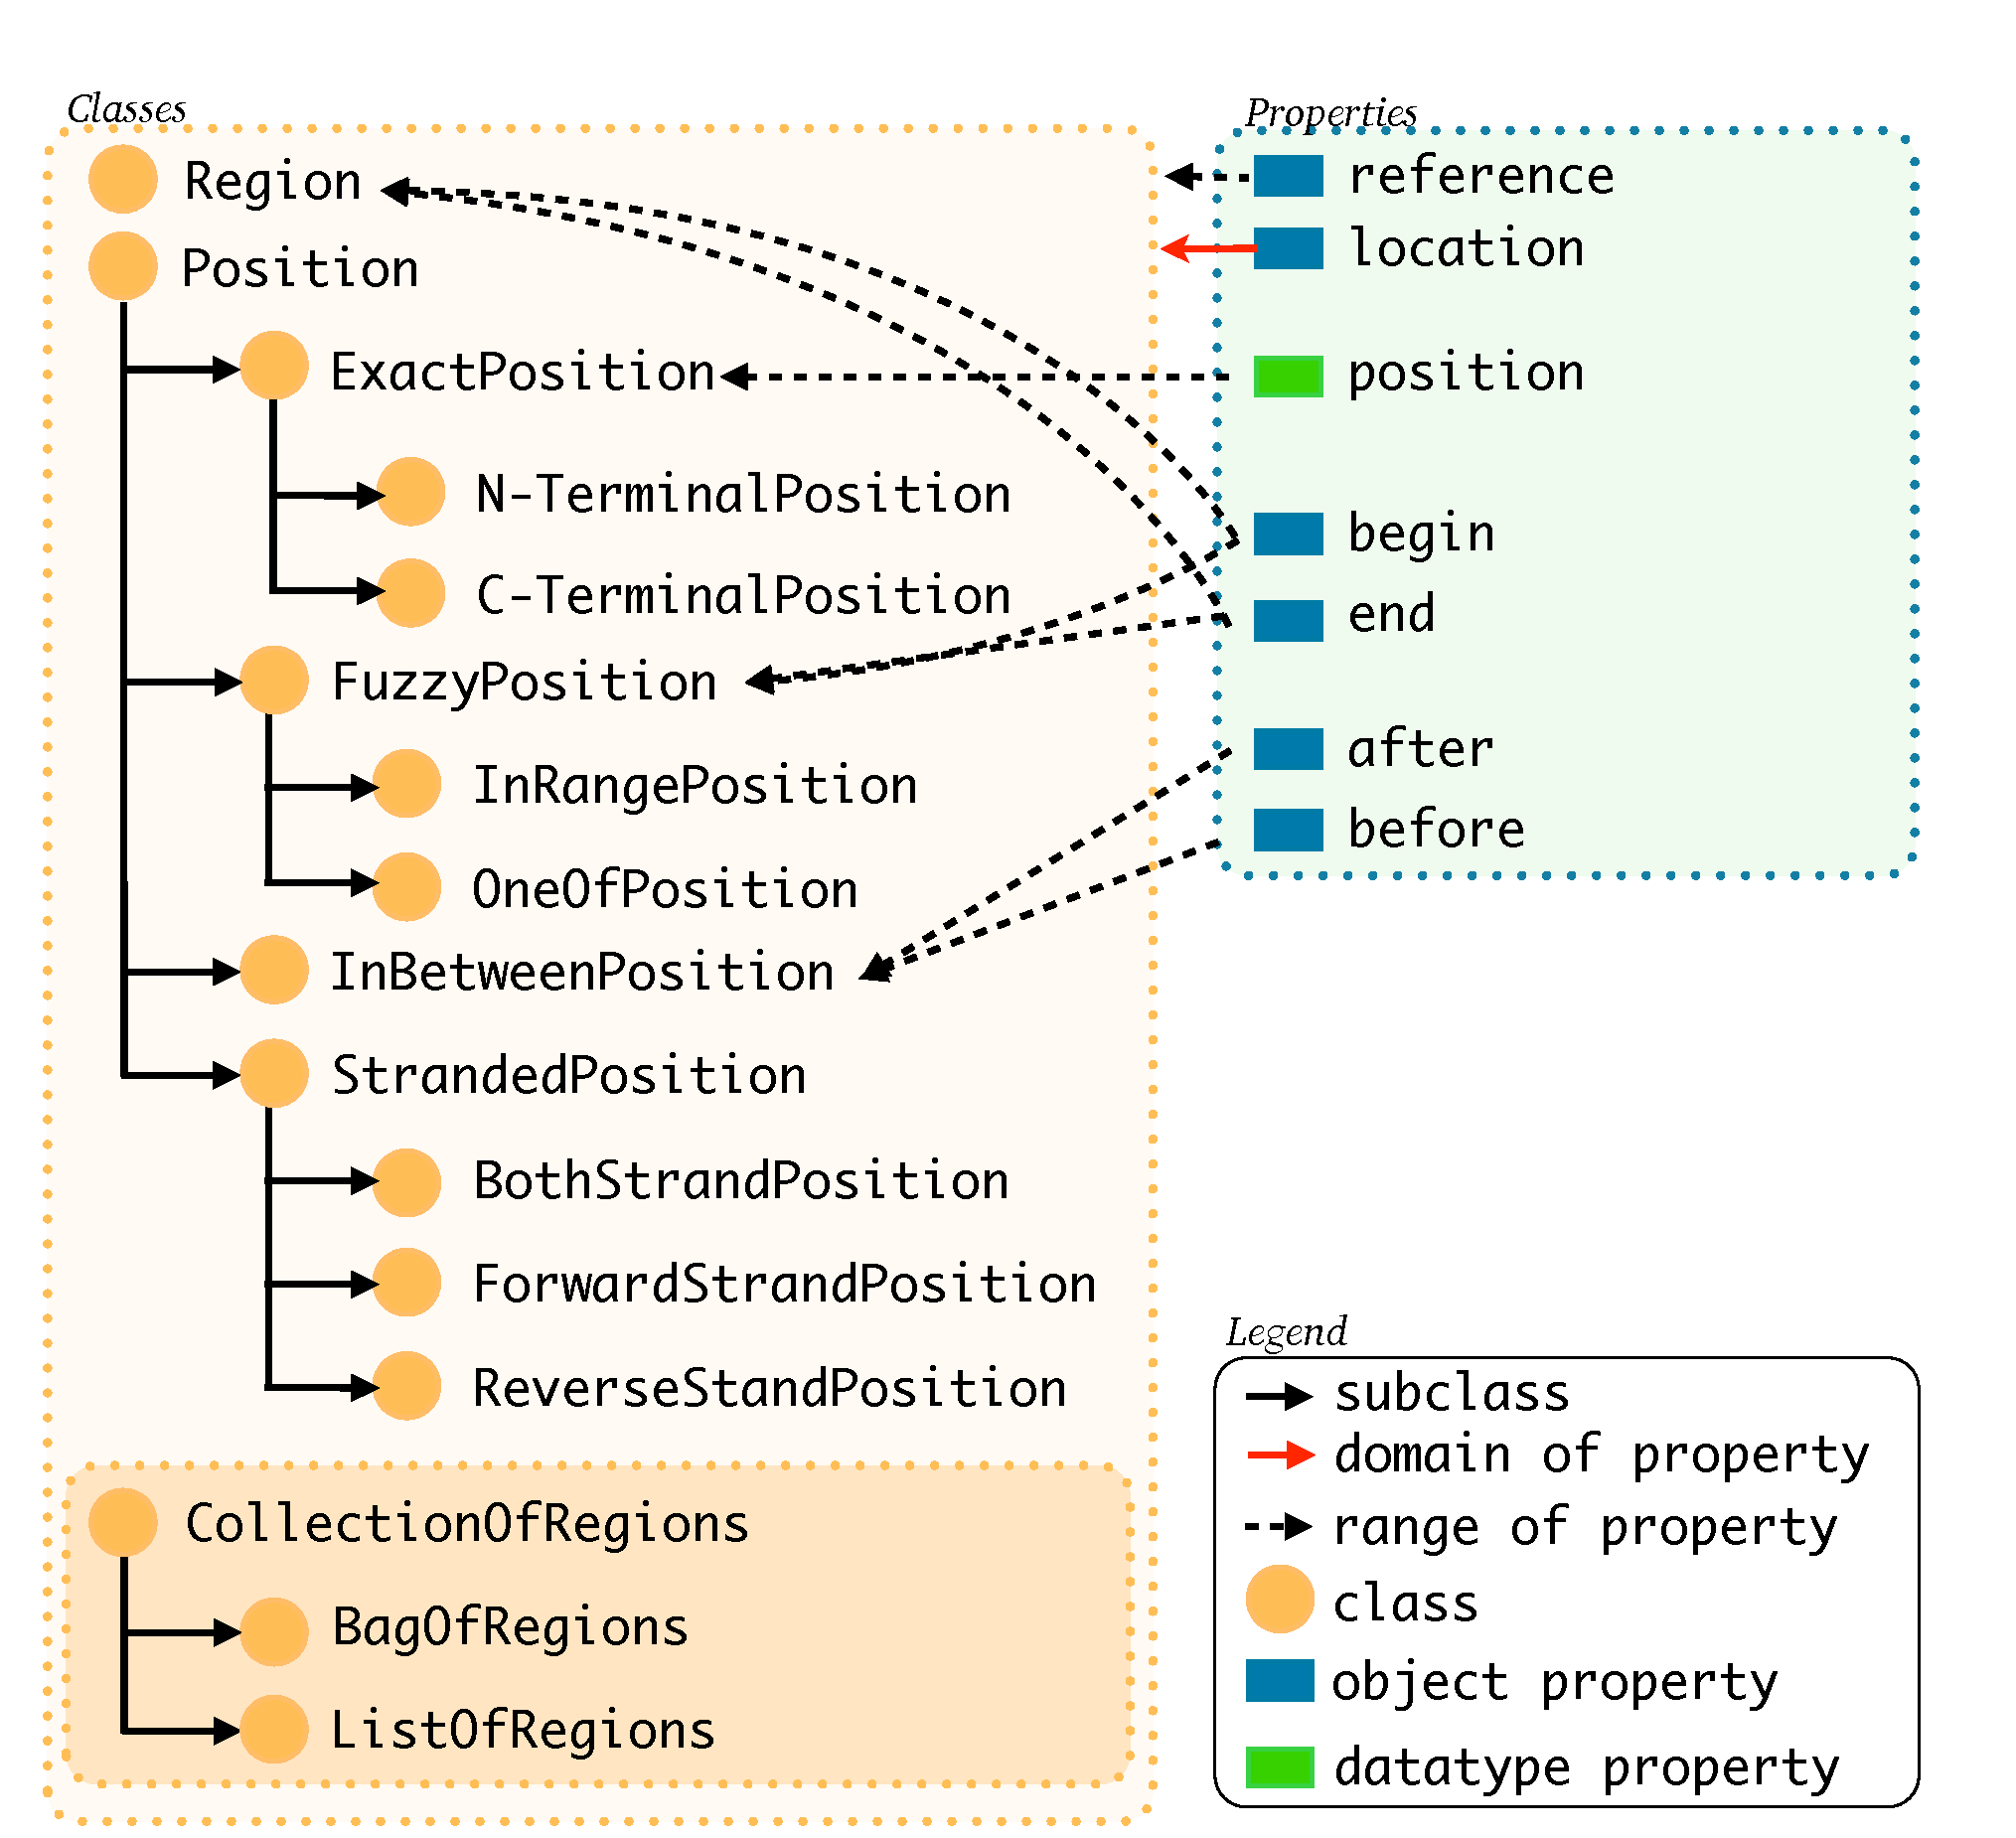
\includegraphics[width=17cm]{figures/ClassDiagram.pdf}
\end{center}
\caption{The classes and object properties used in FALDO.}
\label{fig:ontology}
\end{figure}


\begin{figure}
\begin{center}
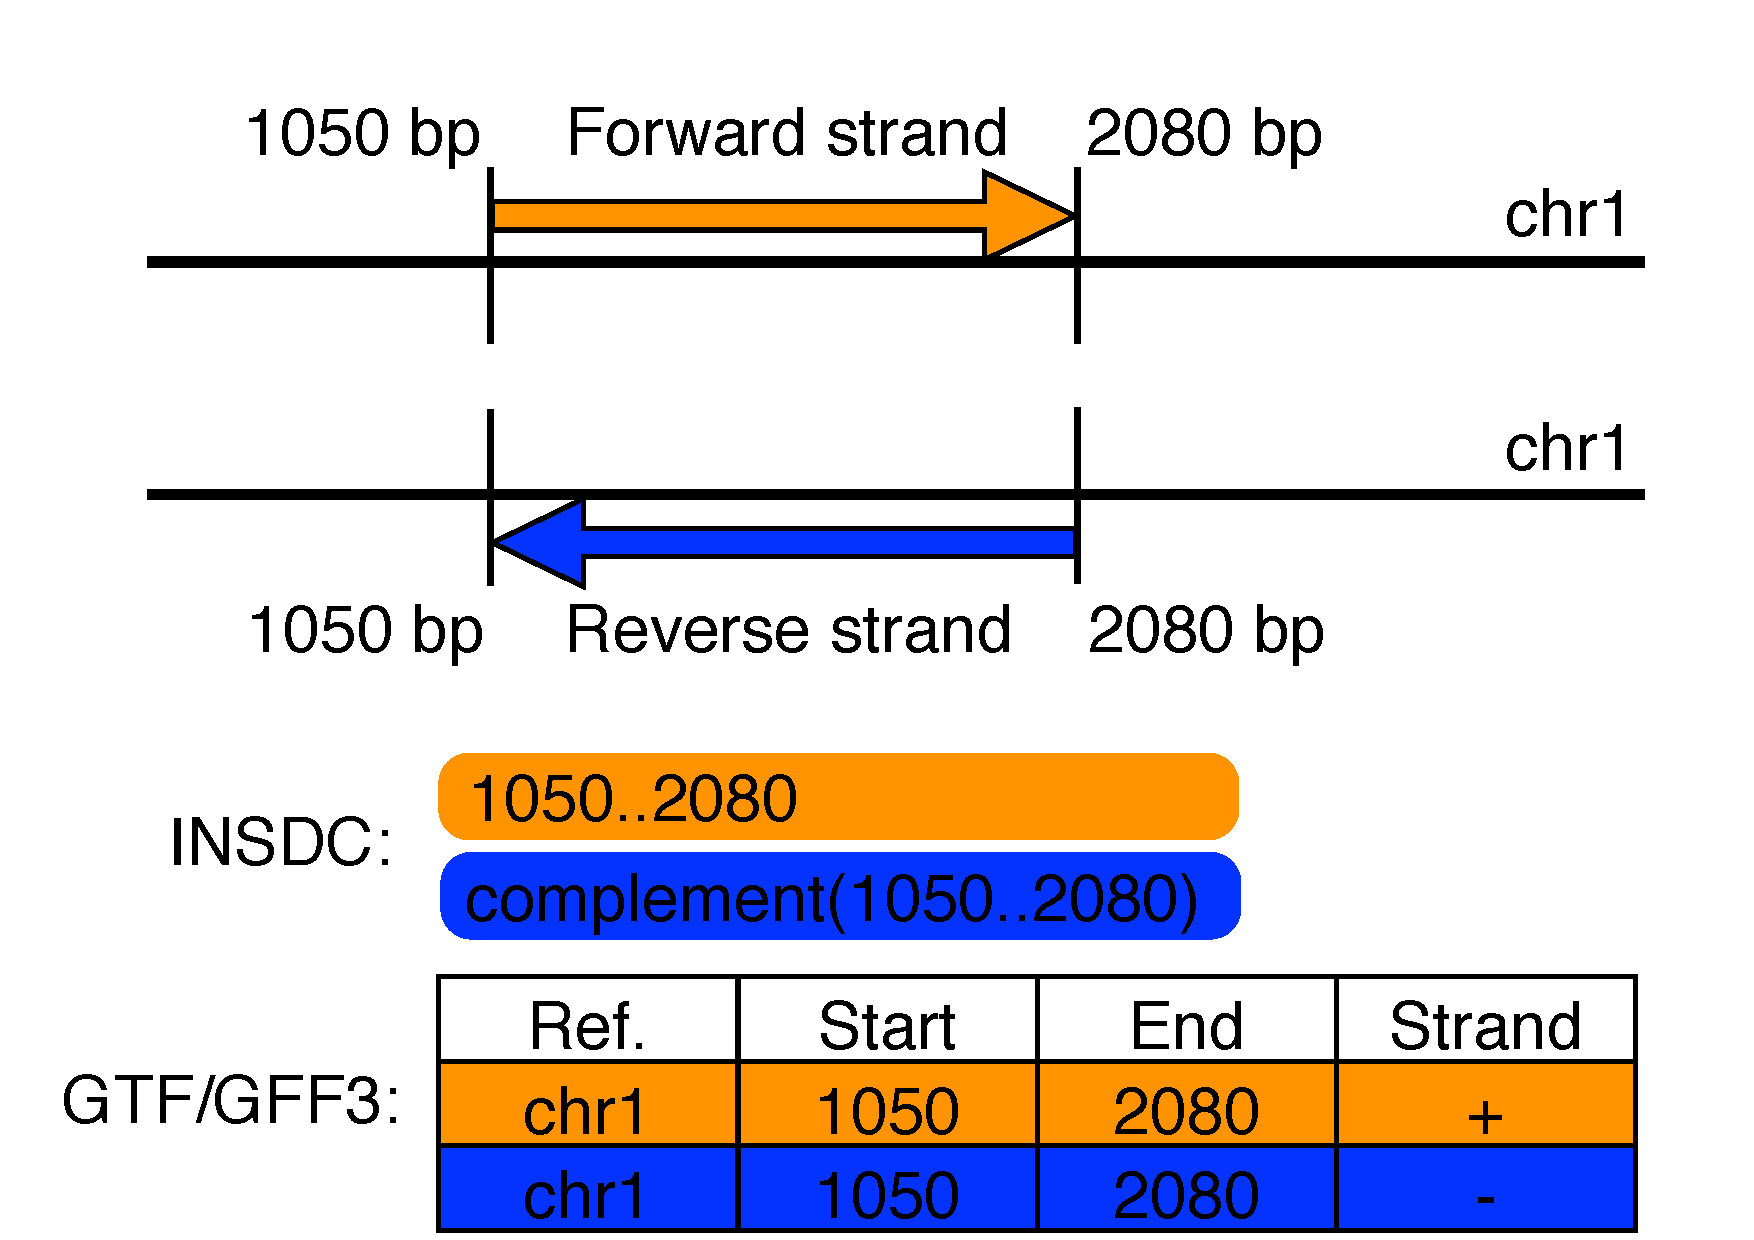
\includegraphics[width=8cm]{figures/figures.pdf}
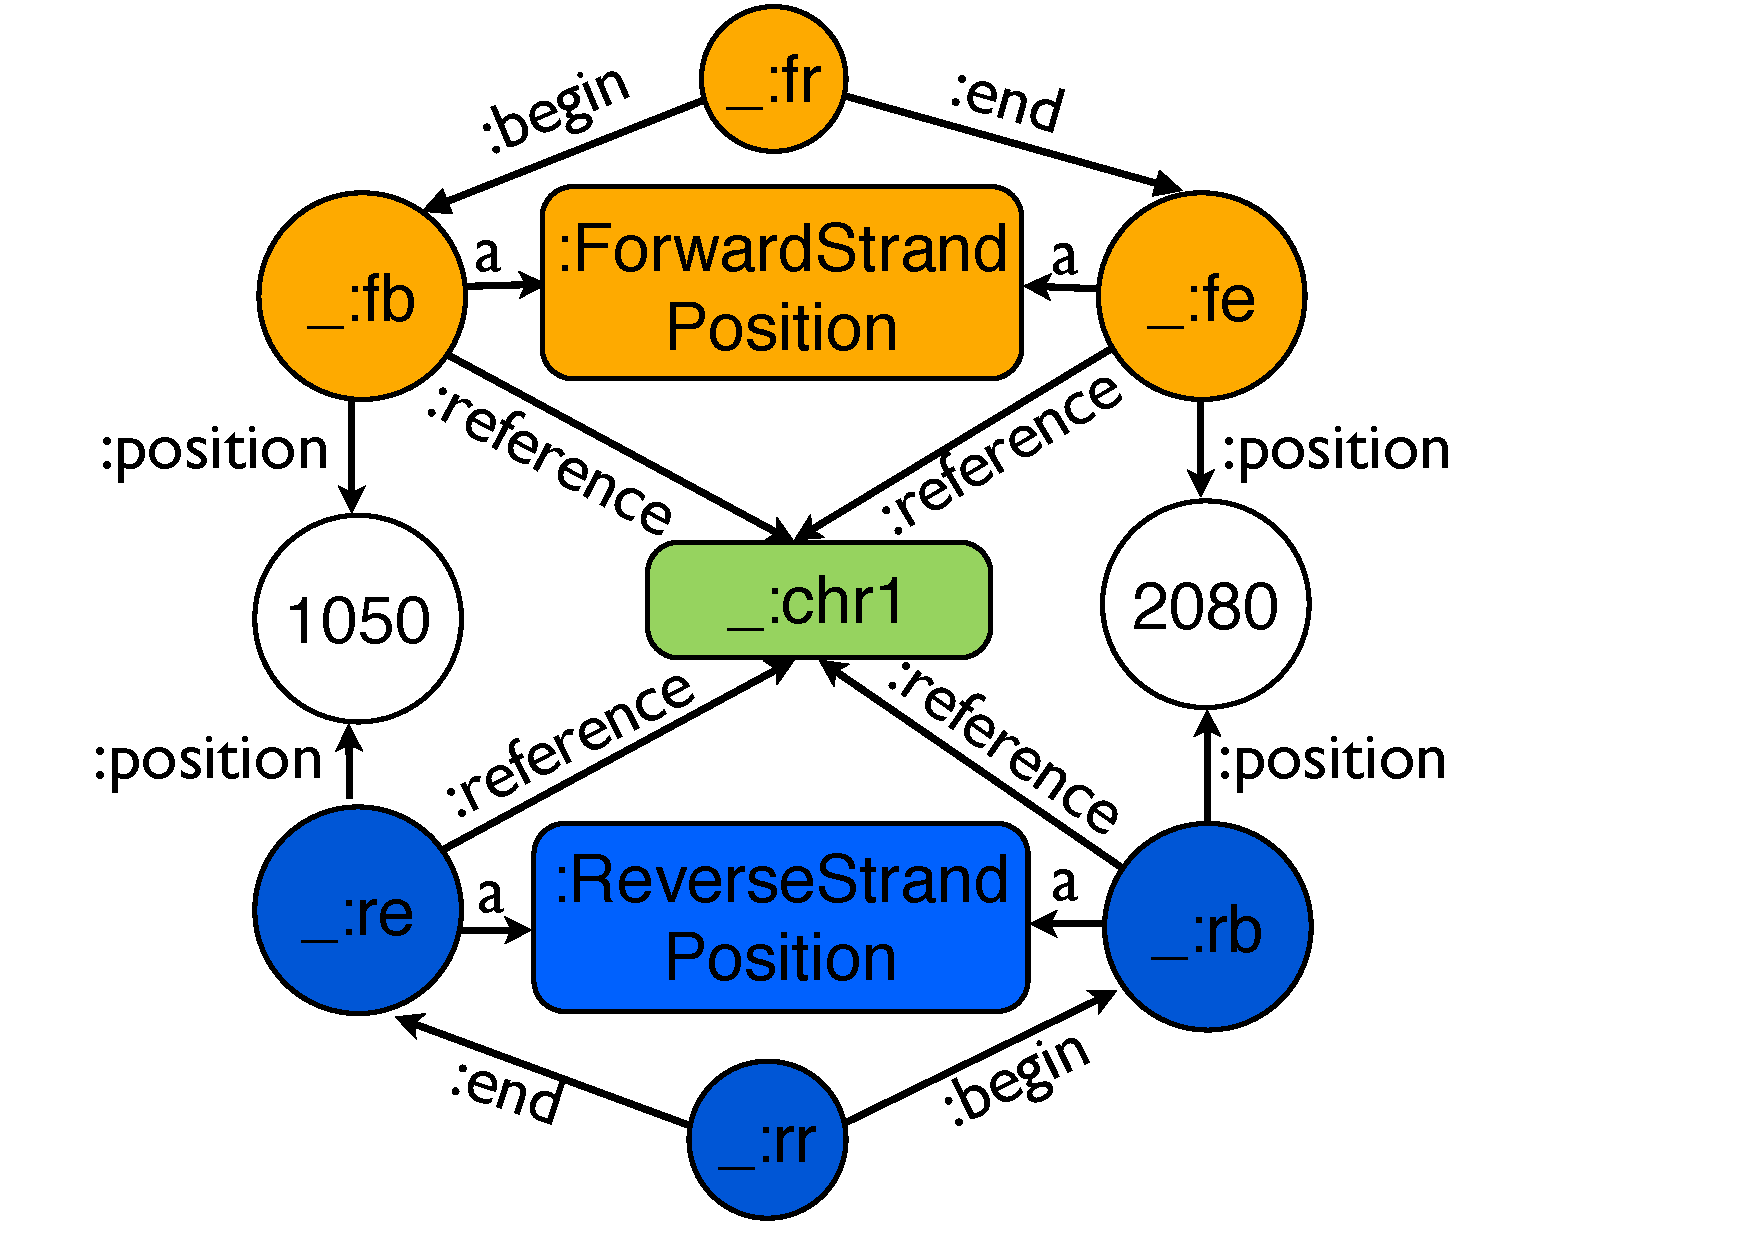
\includegraphics[width=8cm]{figures/figures3.pdf}
\end{center}
\caption{Assorted conventions for regions, start, end, and strands.
This figure shows two hypothetical features on a DNA sequence
(labeled \texttt{chr1}), on either the forward strand (orange) or
reverse strand (blue).
Using the INSDC location string notation, these regions are
``\texttt{1050..2080}'' and ``\texttt{complement(1050..2080)}''
respectively if implicitly given in terms of the reference chr1.
Using the GTF/GFF3 family of formats, regardless of the
strand these two locations are described with $start = 1050$
and $end = 2080$, and in general, $start \leq end$.
Biologically speaking, in terms of transcription, the start of a genomic
feature is strand dependent.
For the forward strand feature (orange), the start is 1050
while the reverse strand feature (blue) starts from 2080.}
\label{fig:strands}
\end{figure}

\subsection*{Easier data integration due to OWL reasoning}

Two $\mathtt{owl\colon{}Class}$es ease dataintgration with a $\mathtt{owl\colon{}hasKey}$ construct. 
A $\mathtt{faldo\colon{}ExactPosition}$ is the same as another position if it has the same $\mathtt{faldo\colon{}position}$ and $\mathtt{faldo\colon{}reference}$.
In practicse this means that if two sequence records are declared to be $\mathtt{owl\colon{}}$ then the features mapped to one of these sequence records is automatically mapped to the other.
i.e. One extra statement allows feature annotation from a UniProt protein record to be transferred to INSDC Coding Domain Features.

\subsection*{Compression via OWL2 reasoning}
For large databases such as INSDC or UniProt,
the need to repeat the reference sequence for each position may come with a significant cost in storage.
However, this triple does not need to be materialised in the database, as it is inferrable using OWL2 property chain reasoning.
With the axiom shown in Figure~\ref{owl:chainProperty} the $\mathtt{faldo\colon{}reference}$ triples can be inferred for any $\mathtt{faldo\colon{}position}$ described by an INSDC record.
Having an OWL-capable query rewriter allows users to ignore the difference between encoding the $\mathtt{faldo\colon{}reference}$ properties explicitly and having them inferred at query time.
For RDF databases that do not offer this capability,
the necessary triples can be easily added using a single SPARQL insert query (Figure~\ref{sparql:chainProperty}).
This flexibility allows users of the data to select the best approach for their infrastructure, rather than being constrained by the decisions of the data provider.

\begin{figure}
\begin{shaded}
\small
\begin{verbatim}
insdc:reference
      a       owl:ObjectProperty ;
      rdfs:subPropertyOf faldo:reference ;
      owl:propertyChainAxiom
              (faldo:endOf faldo:locationOf insdc:featureOf insdc:sequence) , 
              (faldo:locationOf insdc:featureOf insdc:sequence) , 
              (faldo:beginOf faldo:locationOf insdc:featureOf insdc:sequence) .

\end{verbatim}
\end{shaded}
\caption{OWL2 property chain axiom to infer that all positions described in an INSDC record are relative to the main sequence of the record (in RDF turtle syntax, prefixes omitted).}
\label{owl:chainProperty}
\end{figure}

\begin{figure}
\begin{shaded}
\small
\begin{verbatim}
INSERT {
    ?position faldo:reference ?sequence .
}
WHERE {
    ?record a insdc:Entry ;
            insdc:feature ?feature ;
            insdc:sequence ?sequence .
    ?feature faldo:location ?location .
      { ?location faldo:begin|faldo:end ?position . }
    UNION
      { ?location a faldo:Position . }
}
\end{verbatim}
\end{shaded}
\caption{A SPARQL query to add all $\mathtt{faldo\colon{}reference}$ properties to $\mathtt{faldo\colon{}positions}$ described from a $\mathtt{insdc\colon{}record}$.}
\label{sparql:chainProperty}
\end{figure}

\subsection*{Validating data encoded with FALDO}

Some databases only allow a subset of FALDO. 
For example INSDC requires that the start and end of a region are on the same sequence,
while UniProt requires that a feature is described in relation to the reference's canonical isoform.
Yet another database might annotate the location of a glycsoylation site on an UniProt isoform sequence.
When added to an UniProt record in RDF, this extra RDF annotation would be ignored by applications that are not concerned with glycosylation of isoforms.
The same annotation cannot be added to UniProt XML as the XSD schema does not allow for it,
and the older plain text flat-file format does not allow for this kind of third party extension either.
An attempt to add such information would very likely break any XML or flat-file parser and introduces the risk of importing data incorrectly.
Only the UniProt RDF format allows other people to make assertions about UniProt data without breaking existing tools.

There are many ways to add constraints to the data model by applications using Semantic Web technologies\cite{RDFValidationReport}.
In other words, data validation is an application specific concern instead of a data format concern.

\subsection*{Users}
FALDO is already deployed and used in a number of tools and databases, in each case extended with more semantic web data using resource specific ontologies and schemas as well as other semantic standards e.g. the Sequence Ontology.

\begin{figure}
\begin{center}
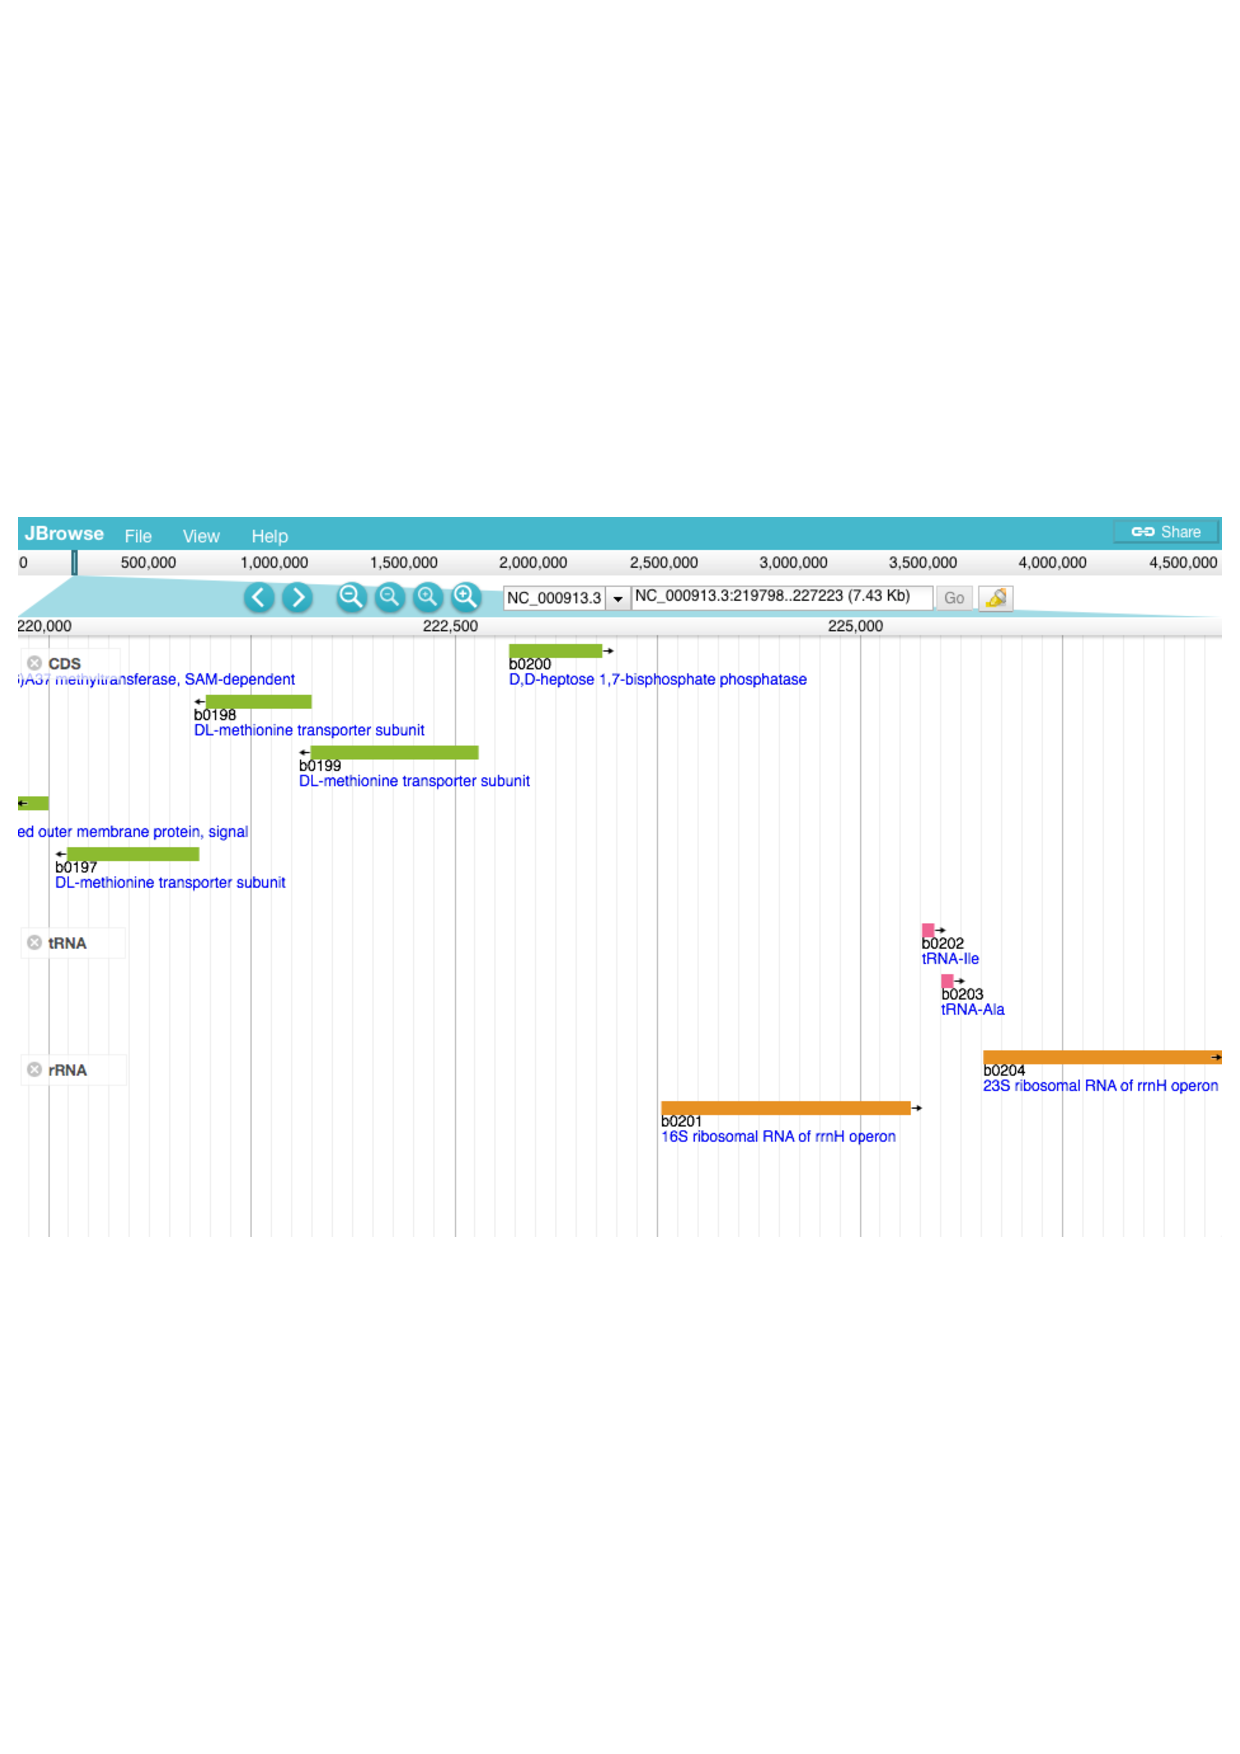
\includegraphics[width=16cm]{figures/togogenomes.pdf}
\end{center}
\caption{JBrowse showing features, whose location is encoded using FALDO, selected via SPARQL (at e.g. \protect\url{http://togogenome.org/gene/1016998:SPAB_00296}). }
\label{fig:jbrowse}
\end{figure}

\begin{description}
\item[JBrowse] can use SPARQL queries with FALDO to visualize annotations on reference sequences from semantic databases \cite{JBrowse} (see Figure \ref{fig:jbrowse}).
\item[INSDC-DDBJ] DDBJ is currently working on an RDF format for the INSDC data that is stored in DDBJ/GenBank/EMBL-Bank.
\item[BioInterchange] uses FALDO to make position information stored in current bioinformatics formats (s.a. GFF3, GTF and GVF) available to the Semantic Web (\url{http://www.biointerchange.org/}).
\item[TogoGenome] a genome database collection provided by the DBCLS also uses FALDO in its RDF representation (\url{http://togogenome.org/}).
%\item[InterMine] The popular model organism database software collection uses FALDO in its SPARQL mode \cite{InterMine}.
\item[PhenomeBrowser] The positions on the mouse genome of phenotype and disease related natural variations are described using FALDO.
\item[BOING] The ``bio-ontology integrated querying of sequence annotations'' framework uses FALDO to describe all feature locations \cite{BOING}.
\item[SPARQL-BED] This simple tool that turns any BED file into a Web accessible SPARQL endpoint using FALDO to describe BED feature positions (\url{https://github.com/JervenBolleman/sparql-bed}).
\item[BioPerl] BioPerl\cite{BioPerl2002} now includes a FALDO exporter (\texttt{Bio::FeatureIO::faldo}), which allows any BioPerl-supported feature format to be translated to FALDO.
\item[UniProt] UniProt annotates many protein features and sites. Starting with UniProt RDF release 2014$\_$01 the positions of protein feature are described using FALDO.
\end{description}


\section*{Results}
One of the practical goal driving the development of FALDO was to be able
to represent all the annotated sequences in UniProt and the INSDC as RDF
triples, as a step towards providing this data via SPARQL end points whereby
it can be queried.
UniProt is already available as RDF, and a revised version of the full
dataset using FALDO has already been tested and is expected to be included
in the UniProt 2013\_11 release \textit{TODO - fill in version and data}.

The protein examples considered, such as the UniProt feature annotations,
require relatively simple locations within protein sequences to be described (see Fig:\ref{fig:UniProt}).
There are corner cases for situations like unknown boundaries for these we use the \mathtt{faldo:InRangePosition}.

\begin{figure}
\begin{verbatim}
AC   P05064;
...
FT   ACT_SITE    230    230       Schiff-base intermediate with
FT                                dihydroxyacetone-P.
\end{verbatim}
\begin{verbatim}
uniprot:P05064 a up:Protein ;
   up:annotation SHA:E50..1B .
SHA:E50..1B a up:Active_Site_Annotation ;
   rdfs:comment ``Schiff-base intermediate with dihydroxyacetone-P''
   faldo:location range:22571003137111085tt230tt230 .
range:22571003137111085tt230tt230 a faldo:Position ;
   faldo:position 230 ;
   faldo:reference isoform:P05064-1 .
\end{verbatim}
\caption{Example from UniProt entry P05064 showing the position of an active site in both faldo and the UniProt flat-file format.}
\label{fig:UniProt}
\end{figure}
\subsection*{Complement strand}
Feature locations on nucleotide sequences can be relatively simple,
%GenBank
for the example (shown in Fig:\ref{fig:insdcComplement}) the \textit{cheY} gene in
\textit{Escherichia coli} str. K-12 substr. MG1655 (accession NC\_000913.2)
is described in the INSDC feature table as \texttt{complement(1965072..1965461)},
which is 390 base pairs using inclusive one-based counting.
This feature begins on the base complementary to $start = 1965461$
and finishes at $end = 1965072$, and so the INSDC location string
can be interpreted as \texttt{complement($end$..$start$)},
FALDO respects this biological interpretation of a feature location
on the reverse strand:

%Notice begin, end = 1965461, 1965072 (biological interpretation)
\begin{figure}
\begin{shaded}
\small
\begin{verbatim}
# 
@prefix faldo: <http://biohackathon.org/resource/faldo#> .

# Here are example triples describing a gene, note the location line:
<_:geneCheY> a so:Gene ;
           rdfs:label "cheY" ;
           faldo:location <_:example> ;

# The following triples define the location used by the feature above,
# made up of a region and its two positions:
<_:example> a faldo:Region ;
           faldo:begin <_:example_b> ;
           faldo:end <_:example_e> .

<_:example_b> a faldo:Position ; 
           a faldo:ExactlyKnownPosition ;
           a faldo:ReverseStrandPosition ;
           faldo:position "1965461"^^xsd:int ;
           faldo:reference refseq:NC_000913.2 .

<_:example_e> a faldo:Position ; 
           a faldo:ExactlyKnownPosition ;
           a faldo:ReverseStrandPosition ;
           faldo:position "1965072"^^xsd:int ;
           faldo:reference refseq:NC_000913.2 .
\end{verbatim}
\end{shaded}
\caption{Incomplete example of using Faldo in turtle format to describe
gene chrY being at complement(NC\_$000913.2:1965072..1965461$)}
\label{fig:insdcComplement}
\end{figure}

In contrast, other formats like GFF require $start \leq end$
regardless of the strand, which is equivalent to interpreting
the INSDC location string as \texttt{complement($start$..$end$)}.
This convention has a number of practical advantages when
dealing with numerical operations on features sets, such as
checking for overlaps or indexing data. For example, the
feature length is given by $length = end - start + 1$ under
this numerically convenient scheme where the interpretation
of $start$ versus $end$ is strand independent.



\subsection*{Compound locations}
Nucleotide data from the INSDC (or GFF3) can require considerably
more complicated sequence locations built out of multiple-regions.

\textit{TODO - examples}.

\subsection*{Fuzzy locations}
Nucleotide data from the INSDC can also require ambiguous end points.

\textit{TODO - examples}.

All of the UniProt protein sequences are now available in RDF format,
with a SPARQL end point currently in beta. Converting more recent
curated INSDC data has been straightforward, however there are a
number of deprecated location strings which have been problematic.
\textit{TODO - examples? manual curation to fix last few oddities?}

\subsection*{Restriction enzymes}

The recognition sites of most restriction enzymes are relatively
straightforward to describe, as is the cleavage site of a blunt
end cutting enzyme \textit{TODO - example of this? Between location}.

However, the cutting point of sticky-end cutting enzymes which
leave an overhang are more challenging to describe. Here the
flexibility in FALDO to allow the start and end positions of a region
to have different strands can be used (Figure~\ref{fig:HindIII}).

\begin{figure}
\begin{framed}
\small
\begin{verbatim}
    \/
5'..AAGCTT..3' 
    123456
3'..TTCGAA..5'
        /\
        
:EnzymeRestrictionSite a example:EnzymeRestrictionSite ;
       faldo:location :EnzymeRestrictionRegion .
       
:EnzymeRestrictionRegion a faldo:Region ;
       faldo:begin :53_1 ;
       faldo:end   :35_6 .
       
:53cleaveageSite a example:CleavageSite ;
       faldo:location :53cleaveageSitePosition .
:35cleaveageSite a example:CleavageSite ;
       faldo:location :35cleaveageSitePosition .
        
:53cleaveageSitePosition a faldo:InBetweenPosition, SO:0001689  ; #five_prime_restriction_enzyme_junction 
       faldo:after :53_1 ;        
       faldo:before :53_2 .
       
:35cleaveageSitePosition a faldo:InBetweenPosition, SO:0001690 ; #three_prime_restriction_enzyme_junction 
       faldo:before :35_5 ;
       faldo:after :35_6 . #Note the before after reversion due to biological start      

       
:53_1 a faldo:ExactPosition , faldo:ForwardStrandedPosition ;
      faldo:position 1 .

:53_2 a faldo:ExactPosition , faldo:ForwardStrandedPosition ;
      faldo:position 2 .

:35_5 a faldo:ExactPosition , faldo:ReverseStrandedPosition ;
      faldo:position 5 .

:35_6 a faldo:ExactPosition , faldo:ReverseStrandedPosition ;
      faldo:position 6 .
\end{verbatim}
\end{framed}
\caption{HindIII restriction enzyme cleavage site with sticky ends}
\label{fig:HindIII}
\end{figure}

Circular genomes bring have number of interesting features to describe. 
The most common is  a feature that straddles the origin of replication or the '0' mark.
For example a gene encoded on the reverse strand of the f1 bacteriophage \textit{todo find accession} which is 6407 base pairs long.
GeneII transcription starts from coordinate 6006 and the transcription ends at position 831.


\subsection*{More examples}

\textit{TODO - other ideas:}
\begin{itemize}
\item Example of Cys bonding between one or two proteins?
\item RNA/DNA digest sites, and the cut sites -- especially for over hangs (start and ends on opposite strands)
\item tRNA hairpin (two complementary regions)?
\item $\beta$-sheet in protein?
\item RNA-Seq mapping (useful for SAM/BAM)?
\end{itemize}



\section*{Discussion}
When designing FALDO, a broad range of use cases were considered from
human genome annotation to glycan binding sites and protein domains on
amino acid sequences, with the goal of developing a scheme general enough
to describe regions of DNA, RNA and protein sequences.

Advantages and drawbacks of existing file formats were considered, including
line based column formats like BED and GTF/GFF which focus on exact
ranges on a given sequence, and the more complex locations supported
by the INSDC feature tables used by GenBank/EMBL/DDBJ.

The simplest non-stranded range location on a linear sequence requires
a start and end coordinate, but even here there are existing competing
conventions for describing open or closed end points using zero and
one based counting (for example BED versus GTF/GFF3/INSDC).

Similarly multiple schemes exist for describing strand specific locations,
with some formats describing features on the reverse strand implicitly
when the start coordinate is numerically higher than the end coordinate
\textit{(TODO - example of format which does this)}.
In FALDO we always count from the start of the forward 5'-3' strand even on the reverse strand.
This encoding means there is no need to know the length of the sequence to compare positions on the different strands.

For a semantic description describing the strand explicitly is preferable.
FALDO chooses to add the strand information to the position. 
This is required to accurately describe for example the sticky ends
of an enzyme digestion cut site, as in the HindIII example (Figure~\ref{fig:HindIII}).

Unlike formats like GTF/GFF3, FALDO shares with Chado the convention
that the start coordinate should be the biological start (which 
may be numerically a higher value than the end coordinate).

A major difference with other proposed standards is that we chose to make strandedness and reference sequence a property of the position instead of the region.
This is important in a number of use cases.
One is when we someone needs to describe the position of a Gene on a rough assembly where the start and end are known to be on a different contig. 
This can be the case when RNA mapping is used in the genome assembly process.
Another is when rough semantics are used in queries e.g. answering what is the start and end of a Gene. 
In a process called transplicing, exons of one gene can be found on multiple chromosomes, or on different strands of the same chromosome. e.g. \textit(TODO find an example)
In such a case the start of the gene is on a different reference sequence or strand than the end.
We encourage that data providers describe the biology more precise than gene start-end in their databases, but we know that legacy data is not easily converted.
Another is Disulfide bonds in a protein complex the start position is on one chain while the end is on another chain in the complex.
FALDO can describe the position of the bridge with InBetweenPositions where the start and end of the bridge is on different protein chains.
This would not be possible if the reference sequence was a property of the region. 
The last difference is that it makes queries more predictable. 
Current formats describe single amino acid binding sites as regions.
FALDO allows us to describe such sites directly on positions therefore the Position class needs the reference sequence property.
For the Region class it is not required as a Region always ends and starts with Positions.

% this could also be integrated with the above rather than forming its own section
\subsection*{Comparison with GMOD/Chado}

The GMOD (Generic Model Organism Database) schema
Chado\cite{Chado2007} includes a module for representing sequences and
sequence features. The Chado model has similarities with RDF in that
the subject-predicate-object pattern is used to represent connections
between biological entities, with community ontologies such as SO used
to type entities and predicates.

Like FALDO, Chado uses the convention that the start position is
always the biological start, even on the reverse strand. Chado allows
multiple locations per feature, but unlike FALDO, the start and end of
any location must be in the same region, which prohibits for example a
feature that spans more than one contig.

The Chado triple pattern is layered on top of a conventional
relational database which leads to inefficiencies when performing many
queries due to the large number of joins required. An RDF store
provides a more natural fit for this kind of model.

\subsection*{Efficiency of Region-of-Interest queries}

Region of interest (ROI) queries are common operations performed on a
set of genome annotations to extract a set of features within a
range. For applications such as genome browsers, it is important that
these are as efficient as possible. Many RDF query engines will
perform poorly when performing ROI queries over large feature
sets. However, we expect that it should be possible to combine
efficient algorithms and indexes such as Nested Containment Lists
(NCLs)\cite{NCL2007} or spatial indexes to optimize these operations
in the context of a SPARQL query.



\subsection*{OWL2 reasoning based compression}
For large databases such as INDSC or UniProt the need to repeat the reference sequence for positions again and again incurs a significant cost in storage.
OWL2 reasoning introduced a new option called PropertyChain reasoning. 
With the axiom shown in fig:\ref{owl:chainProperty} the faldo:reference triples can be inferred for any faldo:position described by a INSDC record.
\begin{figure}
\begin{verbatim}
INDSC:reference
      a       owl:ObjectProperty ;
      rdfs:subPropertyOf faldo:reference ;
      owl:propertyChainAxiom
              (faldo:endOf faldo:locationOf INDSC:featureOf INDSC:sequence) , 
              (faldo:locationOf INDSC:featureOf INDSC:sequence) , 
              (faldo:beginOf faldo:locationOf INDSC:featureOf INDSC:sequence) .

\end{verbatim}
\caption{OWL2 property chain axiom to infer that all positions described in a INSDC record are positioned relative to the main sequence of the record.}
\label{owl:chainProprty}
\end{figure}
A OWL capable query rewriter (e.g. such as part of Stardog) means that users do not see the difference between encoding the faldo:reference explicitly or having them inferred at query time.
Other stores that do not have such capabilities can easily add the necessary triples using a single SPARQL insert query as shown in fig:\ref{sparql:chainProperty}.
\begin{figure}
\begin{verbatim}
CONSTRUCT {
    ?position faldo:reference ?sequence .
}
WHERE {
    ?record a insdc:Entry .
    ?record insdc:feature ?feature .
    ?feature faldo:location ?location .
    {
        ?location faldo:begin|faldo:end ?position .
    }
    UNION
    {
        ?location a faldo:Position .
    } .
    ?record insdc:sequence ?sequence .
}
\end{verbatim}
\caption{SPARQL query to add all faldo:reference properties to faldo:positions described from a insdc:record.}
\label{sparql:chainProperty}
\end{figure}

FALDO has been designed to be open to extension for future use.
To avoid unnesecarry contradictions we avoid stating that a position is unknown.
i.e. a missing triple means unknown. 
This means that a new datasource with more specific information is not contradicted e.g.
we never get $\_:position a :faldo:ExactPosition,faldo:UnknownPosition$ when merging rdf sources.



\section*{Conclusions}
FALDO is a simple and minimalistic ontology for describing biological features in a consistent manner that Bio-informaticians can depend upon.
The diverse software and databases using FALDO show that it has enough power to describe all biological feature positions.
It is now much easier for users querying biological databases on the semantic web to compare features on the basis of locations.
This also means that visualisation tools that access position data via SPARQL can easily reuse significant parts of queries between databases.
\section*{Availability and requirements}
FALDO is publicly available at the URL \url{http://biohackathon.org/resource/faldo}
which is developed under source code control at
\url{https://github.com/JervenBolleman/FALDO} hosted by GitHub Inc.
FALDO currently uses the Creative Commons Attribution 3.0 Unported licence,
making FALDO available to use and reuse free of charge.

The ontology is written using the Turtle (Terse RDF Triple Language) format,
which can be automatically converted to another format such as RDF/XML
if required.





\section*{List of abbreviations}

\begin{description}
\item[SPARQL] SPARQL Protocol and RDF Query Language
\item[UniProtKB] Universal Protein Knowledgebase 
\item[RDF] Resource Description Framework
\item[DNA] Deoxyribonucleic acid
\item[INSDC] International Nucleotide Sequence Database Collaboration
\item[DDBJ] DNA Data Bank of Japan
\item[EMBL] European Molecular Biology Laboratory
\item[ENA] European Nucleotide Archive
\item[BED] Browser Extensible Data (file format)
\item[GTF] Gene Transfer Format
\item[GFF] Generic Feature Format
\item[GFF3] Generic Feature Format version 3
\item[OWL] Web Ontology Language (note acronym is OWL, not WOL)
\end{description}
\bigskip

\section*{Authors contributions}

Jerven Bolleman wrote the basic ontology file and mapping to UniProt RDF and contributed to the text of this article.
Robert Hoehndorf did the GFF3 to OWL conversion.
Peter Cock wrote a large section of this paper.
Raoul JP Bonnal adapted BioRuby to match the ontology and wrote the cufflink to locations.rdf converter with Francesco Strozzi.
Takatomo Fujisawa and Toshiaki Katayama implemented the DDBJ RDF in terms of this format and used FALDO to describe features on bacterial genomes in TogoGenome.
Robert Buels adapted JBrowse to query SPARQL endpoints that use this format to generate custom tracks. 

\section*{Acknowledgments}
The developers recognize the invaluable contributions from the community in helping to create this standard.
This work has been supported by National Bioscience Database Center (NBDC) of Japan Science and Technology Agency (JST) and Database Center for Life Science (DBCLS) of Research Organization of Information and Systems (ROIS) in Japan.
Jerven Bolleman was supported in his role at Swiss-Prot, whose activities at the SIB Swiss Institute of Bioinformatics are supported by the Swiss Federal Government through the The State Secretariat for Education, Research and Innovation SERI.
Christopher Mungall was supported by the NIH under R24OD011883 and by the Director, Office of Science, Office of Basic Energy Sciences, of the U.S. Department of Energy under Contract No. DE-AC02-05CH11231.
Peter Cock was supported by the Scottish Government Rural and Environmental Research and Analysis Directorate.
Takatomo Fujisawa was supported by the DNA Databank of Japan (DDBJ), Research Organization of Information and Systems (ROIS) in Japan.

\newpage
{\ifthenelse{\boolean{publ}}{\footnotesize}{\small}
 \bibliographystyle{bmc_article}  % Style BST file
  \bibliography{locations} }     % Bibliography file (usually '*.bib' ) 
  
\end{bmcformat}
\end{document}
